\chapter{DESAIN DAN IMPLEMENTASI}
\label{chap:desainimplementasi}

% Ubah bagian-bagian berikut dengan isi dari desain dan implementasi

Penelitian ini dilaksanakan sesuai dengan desain sistem berikut dengan implementasinya. Desain sistem merupakan konsep dari pembuatan dan perancangan infrastruktur dan kemudian diwujudkan dalam bentuk blok-blok alur yang harus dikerjakan. Metodologi dari sistem yang dikerjakan dalam penelitian ini dapat dilihat pada blok diagram berikut

\begin{figure}[ht]
	\centering
	
	% Ubah dengan nama file gambar dan ukuran yang akan digunakan
	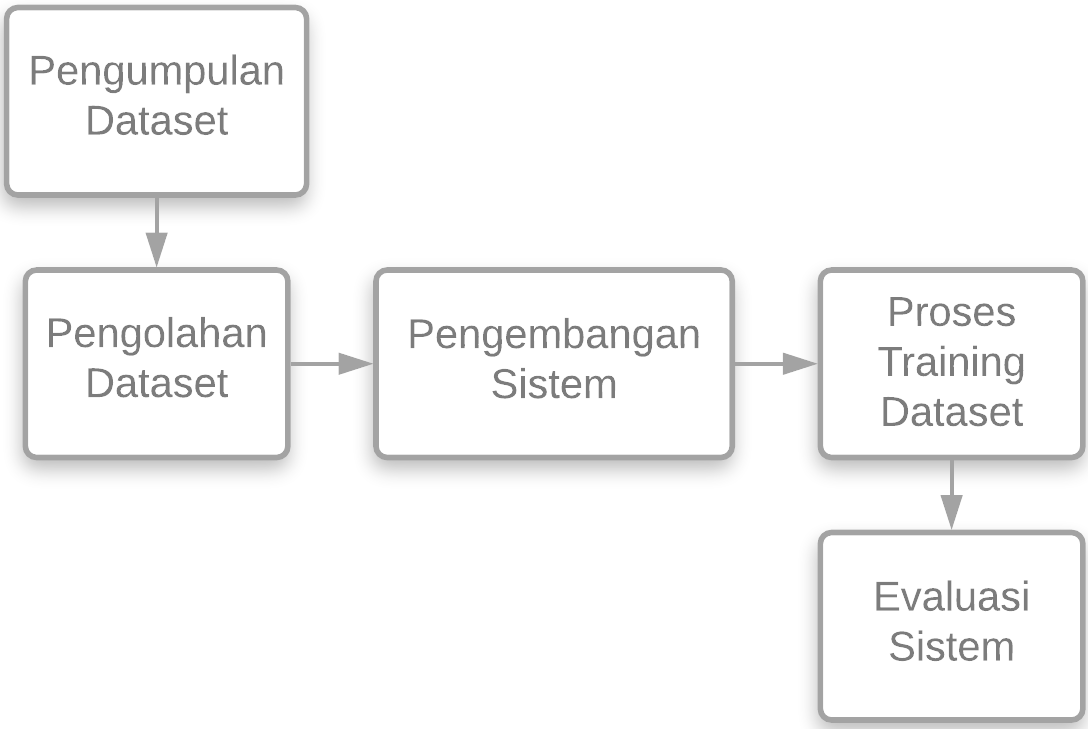
\includegraphics[width=0.7\columnwidth]{gambar/AlurKerja.png}
	
	% Ubah dengan keterangan gambar yang diinginkan
	\caption{Alur Kerja}
	\label{fig:blokdiagram}
\end{figure}

\section{Desain Sistem}
\label{sec:desasinsistem}

Tugas akhir ini merupakan penelitian dalam bidang visi komputer yang bertujuan untuk mendeteksi gerakan mencuci tangan dengan memanfaatkan teknologi \textit{Deep Learning} Berbasis \textit{Convolutional Neural Network (CNN))}. Sistem deteksi ini dilatih menggunakan data training yang diambil dari kaggle (Sample: Handwash Dataset \cite{cit:kaggledata}) ditambahkan dengan dataset yang penulis kumpulkan secara pribadi. 

\section{Alur Kerja}
\label{sec:alurkerja}

Alur implementasi dalam pengerjaan penelitian ini dibagi menjadi beberapa tahapan berdasarkan metodologi penelitian, yaitu: 
\begin{enumerate}[noitemsep]
	\item Pengumpulan Dataset
	\item Pengolahan Dataset
	\item Pengembangan Sistem
	\item Proses Training Dataset
	\item Evaluasi Sistem
\end{enumerate}

\section{Pengumpulan Dataset}
\label{sec:pengumpulandata}

Sebagian besar dataset yang digunakan pada penelitian ini berasal dari Kaggle \cite{cit:kaggledata}. isi dari dataset ini dapat dilihat pada tabel \ref{tab:kagglelist}
% Please add the following required packages to your document preamble:
% \usepackage{graphicx}
\begin{table}[!ht]
	\centering
	\resizebox{0.9\textwidth}{!}{%
		\begin{tabular}{|l|l|c|}
			\hline
			\multicolumn{1}{|c|}{Class} & \multicolumn{1}{c|}{Description}      & \#Videos \\ \hline
			Step 1                      & Rubbing Palm Together                 & 25       \\ \hline
			Step 2 Left                 & Rub Palm Over Dorsum                  & 25       \\ \hline
			Step 2 Right                & Rub Palm Over Dorsum                  & 25       \\ \hline
			Step 3                      & Rubbing Palm With Fingger Interlanced & 25       \\ \hline
			Step 4 Left                 & Rub Nails on Palm                     & 25       \\ \hline
			Step 4 Right                & Rub Nails on Palm                     & 25       \\ \hline
			Step 5 Left                 & Rub Between Thumb and Index Fingger   & 25       \\ \hline
			Step 5 Right                & Rub Between Thumb and Index Fingger   & 25       \\ \hline
			Step 6 Left                 & Rub Finggertips on Palm               & 25       \\ \hline
			Step 6 Right                & Rub Finggertips on Palm               & 25       \\ \hline
			Step 7 Left                 & Rub Thumb                             & 25       \\ \hline
			Step 7 Right                & Rub Thumb                             & 25       \\ \hline
		\end{tabular}%
	}
	\caption{Isi Hand Wash Dataset Kaggle}
	\label{tab:kagglelist}
\end{table}

Pada dataset tersebut, ditemukan berberapa kesalahan seperti kesalahan \textit{labeling}, kesalahan pengelompokan file dan noise berupa video yang \textit{"terkontaminasi"} gerakan berbeda didalamnya, oleh sebab itu dataset ini memerlukan pengecekan dan pemrosesan lebih lanjut agar dapat digunakan pada tahap training. Tidak diketahui spesifikasi kamera yang digunakan dalam pengambilan dataset ini. Sample dari dataset ini dapat dilihat pada gambar \ref{fig:sampledata}

\begin{figure}[!ht]
	\centering
	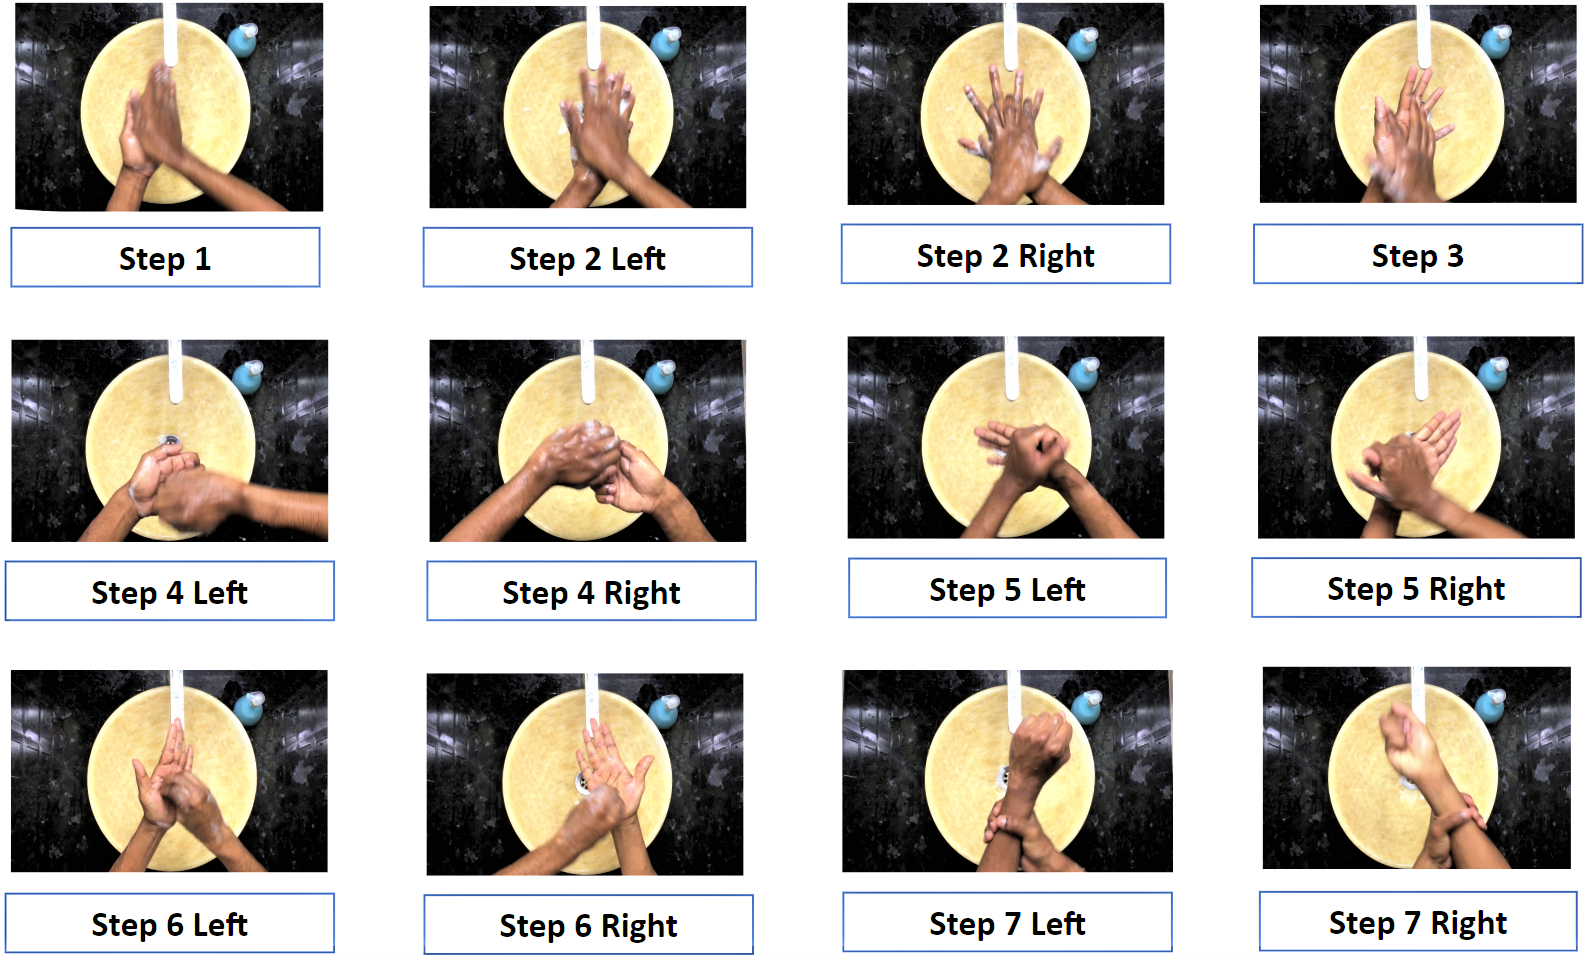
\includegraphics[width=0.9\columnwidth]{gambar/sampledatasetkaggle.png}
	\caption{Sampel dataset Kaggle\cite{cit:kaggledata}}
	\label{fig:sampledata}
\end{figure}

Penulis juga menambahkan dataset pribadi guna melakukan pengujian lebih lanjut. Dataset dikumpulkan dengan 2 kamera berbeda guna mengetahui pengaruh sudut, \textit{background}, serta distorsi lensa pada hasil klasifikasi.

Pengambilan dataset pribadi yang pertama dilakukan di tempat tinggal penulis menggunakan kamera \textit{webcam M-Tech WB-500}. Spesifikasi webcam ini dapat dilihat pada tabel \ref{tab:wb500}
\begin{table}[!ht]
	\centering
	\resizebox{0.6\textwidth}{!}{%
		\begin{tabular}{|l|c|}
			\hline
			\multicolumn{2}{|c|}{Spesifikasi Webcam M-Tech WB-500} \\ \hline
			Maximum Resolution         & 1080p/30fps               \\ \hline
			Image Sensor               & CMOS                      \\ \hline
			Focus Type                 & Fixed Focus               \\ \hline
			Lens                       & 3P                        \\ \hline
			Field of View              & 69°                       \\ \hline
			Microphone                 & Digital                   \\ \hline
			Interface                  & High Speed USB 2.0        \\ \hline
		\end{tabular}%
	}
	\caption{Spesifikasi M-Tech WB-500 \cite{cit:wb500}}
	\label{tab:wb500}
\end{table}

\textit{Setup} pengambilan dataset ini dapat dilihat pada gambar dan contoh video yang didapatkan dapar di lihat pada gambar \ref{fig:webcam2} dan gambar \ref{fig:contohwebcam}

\begin{figure}[!ht]
	\centering
	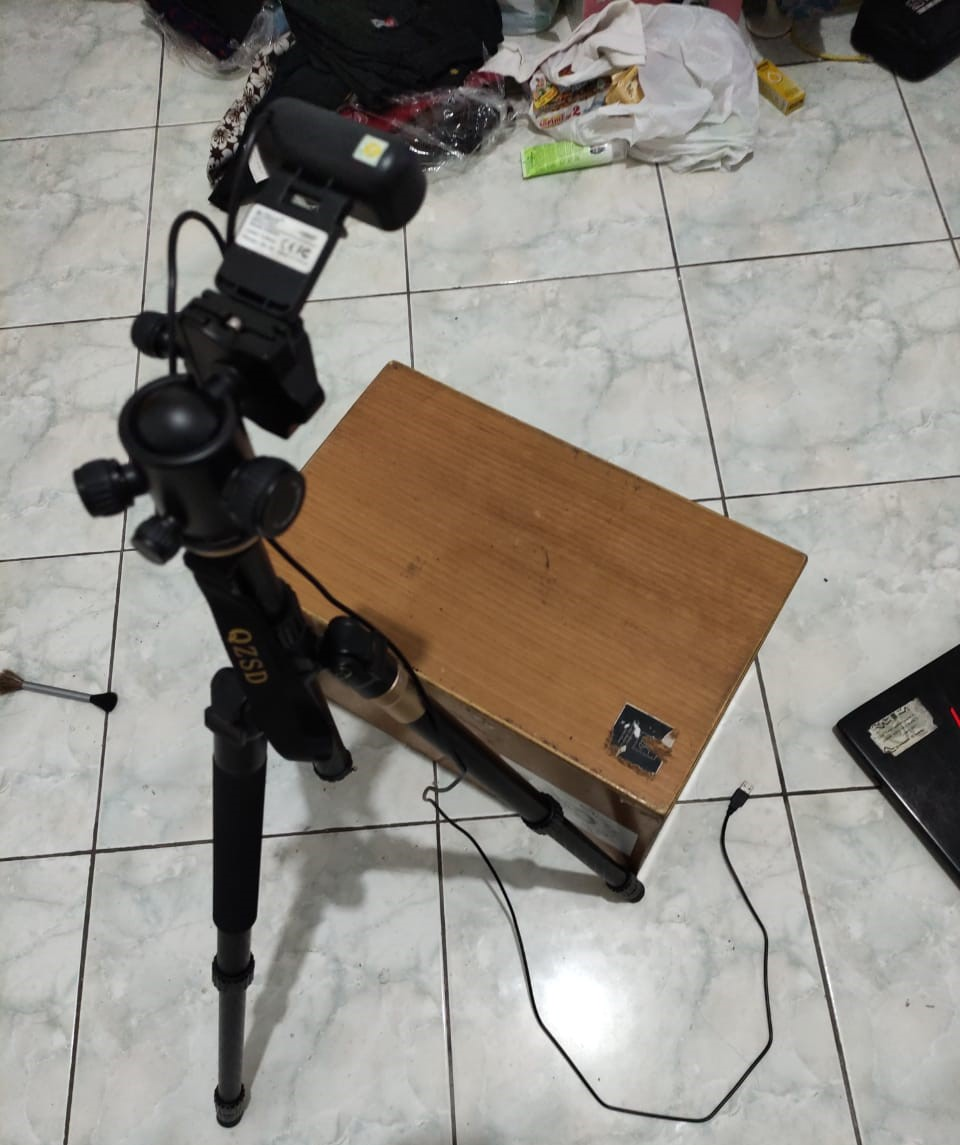
\includegraphics[width=0.67\columnwidth]{gambar/webcam2.jpeg}
	\caption{Setup pengambilan dataset menggunakan webcam}
	\label{fig:webcam2}
\end{figure}

\begin{figure}[!ht]
	\centering
	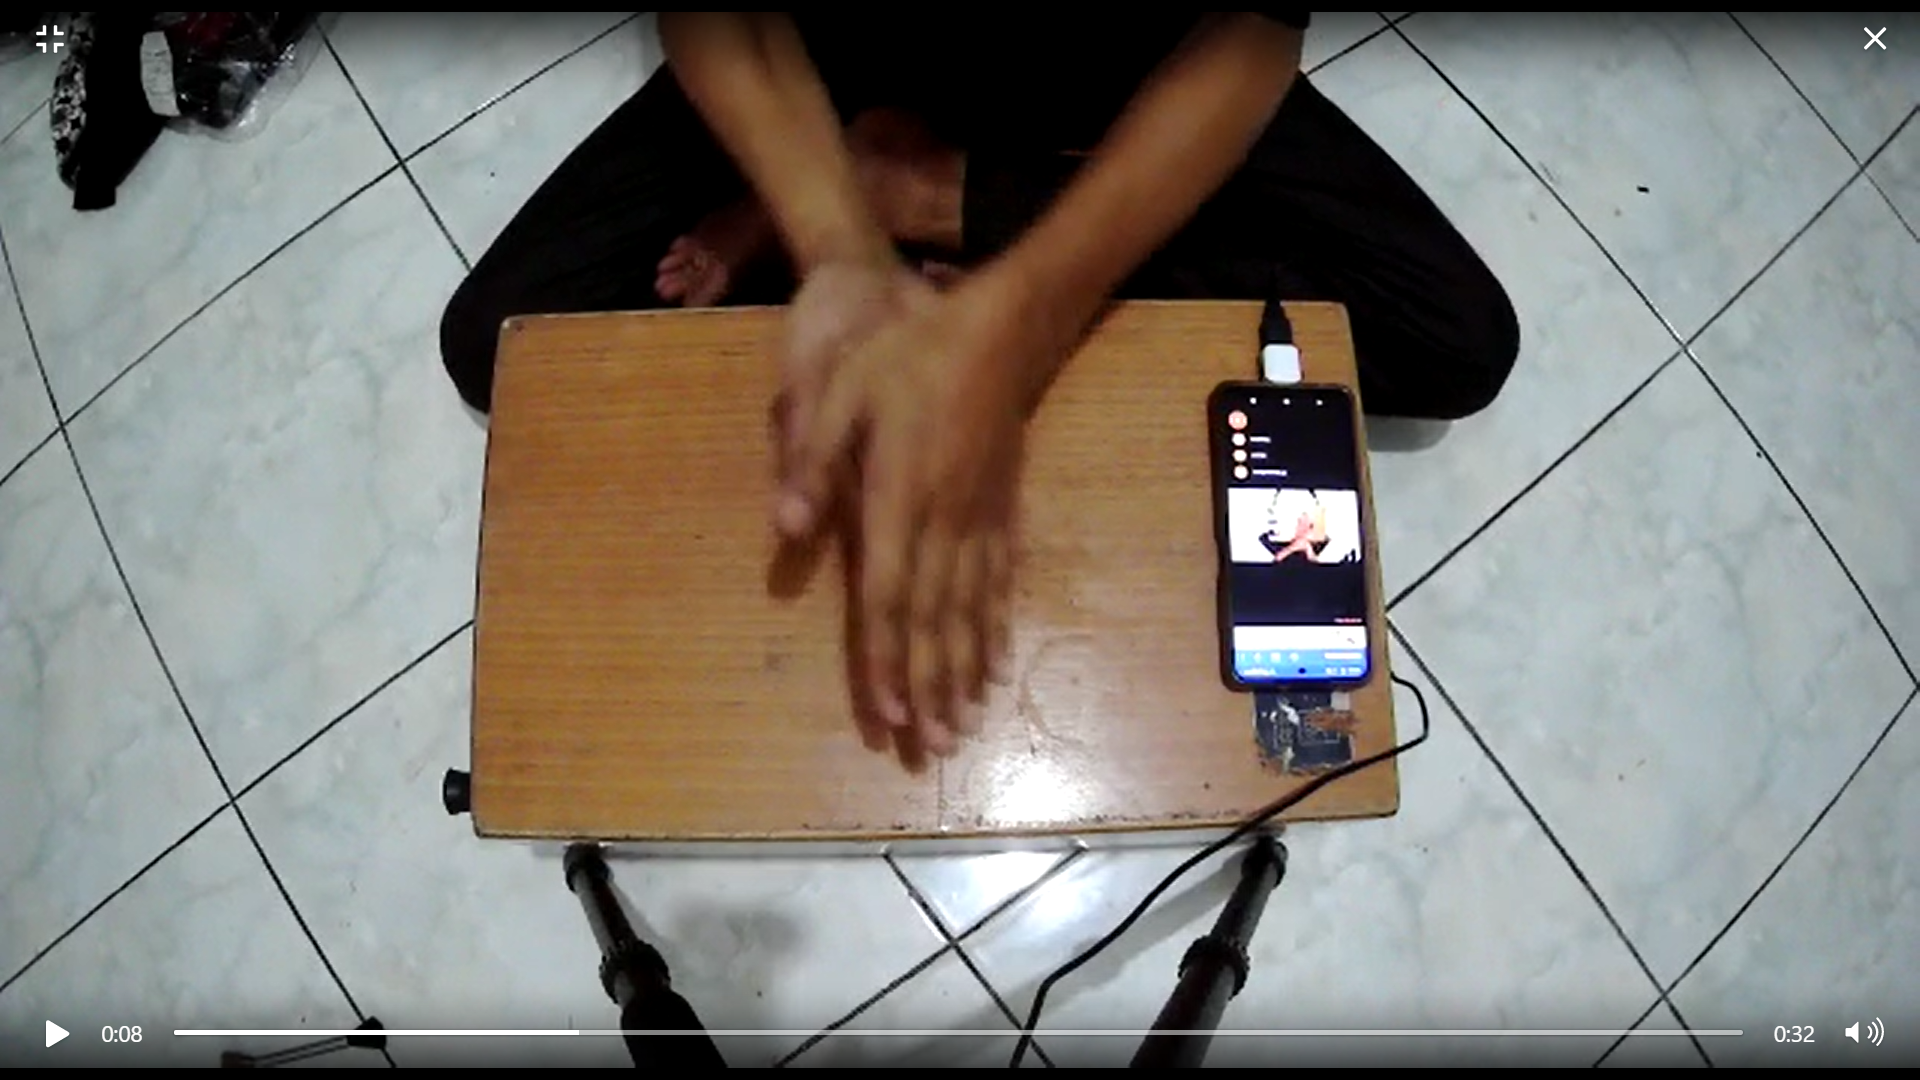
\includegraphics[width=0.85\columnwidth]{gambar/contohwebcam1.png}
	\caption{Contoh hasil video webcam}
	\label{fig:contohwebcam}
\end{figure}

Pengambilan dataset pribadi yang kedua dilakukan di wilayah kampus ITS, tepatnya di gedung laboratorium AJ Elektro. Dataset video ini diambil menggunakan Kamera \textit{DSLR} yang ditempatkan diatas tripod dan diarahkan ke wastafel. Spesifikasi kamera, lensa, dan konfigurasi yang digunakan dapat dilihat pada tabel \ref{tab:canon100d}, \ref{tab:1855stm} dan tabel \ref{tab:pengaturandslr}

\begin{table}[!ht]
	\centering
	\resizebox{0.7\textwidth}{!}{%
		\begin{tabular}{|c|c|}
			\hline
			\multicolumn{2}{|c|}{\textbf{Spesifikasi Dasar Canon EOS 100D}} \\ \hline
			Sensor            & 18 MP APS-C CMOS Sensor                     \\ \hline
			Processor         & DIGIC 5 Image Processor                     \\ \hline
			Display           & 3" 1.04m Dot Clear-View II Touchscreen      \\ \hline
			Video Resolution  & Full HD 1080p Video Recording at 30 fps     \\ \hline
			Auto Focus        & 9-Point AF and Hybrid CMOS AF II            \\ \hline
			ISO               & Native ISO 12800, Extended to ISO 25600     \\ \hline
			Shutter           & 4 fps Shooting for 28 JPEG, 7 Raw Files     \\ \hline
			Metering          & 63-Zone Dual-Layer Metering System          \\ \hline
		\end{tabular}%
	}
	\caption{Spesifikasi Canon EOS 100D \cite{cit:100d}}
	\label{tab:canon100d}
\end{table}

\begin{table}[!ht]
	\centering
	\resizebox{1\textwidth}{!}{%
		\begin{tabular}{|l|l|}
			\hline
			\multicolumn{2}{|c|}{\textbf{Spesifikasi Lensa EF-s 18-55mm f/3.5 - 5.6 IS STM}}                \\ \hline
			Image size                             & APS-C          \\ \hline
			35mm film equivalent focal length (mm) & 29-88          \\ \hline
			Angle of view (horzntl, vertl, diagnl) & 64º 30' - 23º 20', 45º 30'- 15º 40', 74º 20' - 27º 50' \\ \hline
			Lens construction (elements/groups)    & 13/11          \\ \hline
			No. of diaphragm blades                & 7              \\ \hline
			Minimum aperture                       & 22 - 38(36)¹   \\ \hline
			Closest focussing distance (m)         & 0.25           \\ \hline
			Maximum magnification (x)              & 0.36 (at 55mm) \\ \hline
			Distance Information                   & Provided       \\ \hline
			Image stabilizer                       & 4-stops        \\ \hline
			AF actuator                            & STM            \\ \hline
		\end{tabular}%
	}
	\caption{Spesifikasi Lensa EF-s 18-55mm f/3.5 - 5.6 IS STM}
	\label{tab:1855stm}
\end{table}

\begin{table}[!ht]
	\centering
	\resizebox{0.6\textwidth}{!}{%
		\begin{tabular}{|l|l|}
			\hline
			\multicolumn{2}{|c|}{\textbf{Pengaturan Perekaman Kamera DSLR}} \\ \hline
			Resolution                        & 720p 60FPS                  \\ \hline
			Frame Rate                        & 60FPS                       \\ \hline
			Zoom                              & 18mm                        \\ \hline
			Aperture                          & Auto                        \\ \hline
			Focussing                         & Auto Focus                  \\ \hline
			Shutter Speed                     & 60                          \\ \hline
			Image Stablilzer                  & On (Lens)                   \\ \hline
		\end{tabular}%
	}
	\caption{Pengaturan Perekaman Kamera DSLR}
	\label{tab:pengaturandslr}
\end{table}

Setup pengambilan dan contoh hasil video dapat dilihat pada gambar \ref{fig:setupdslr} dan gambar \ref{fig:contohdslr}

\begin{figure}[!ht]
	\centering
	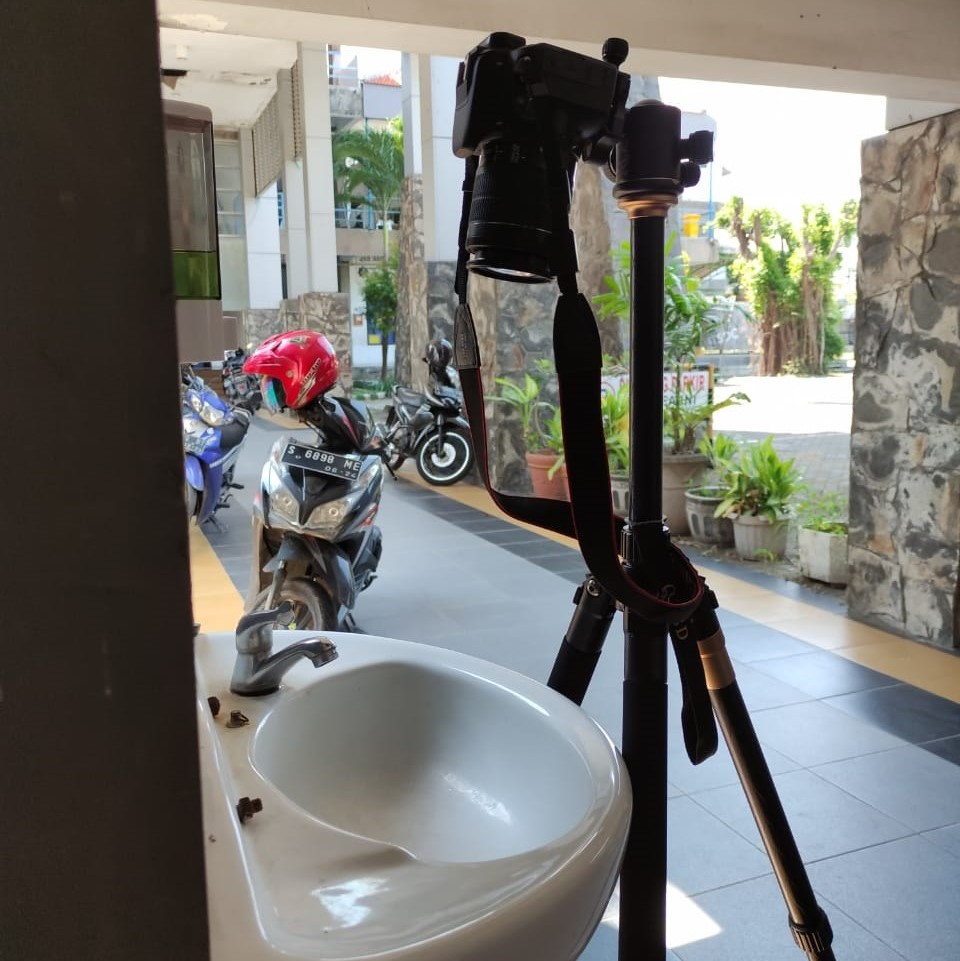
\includegraphics[width=0.65\columnwidth]{gambar/setupdata2.jpeg}
	\caption{Contoh hasil Video DSLR}
	\label{fig:setupdslr}
\end{figure}

\begin{figure}[!ht]
	\centering
	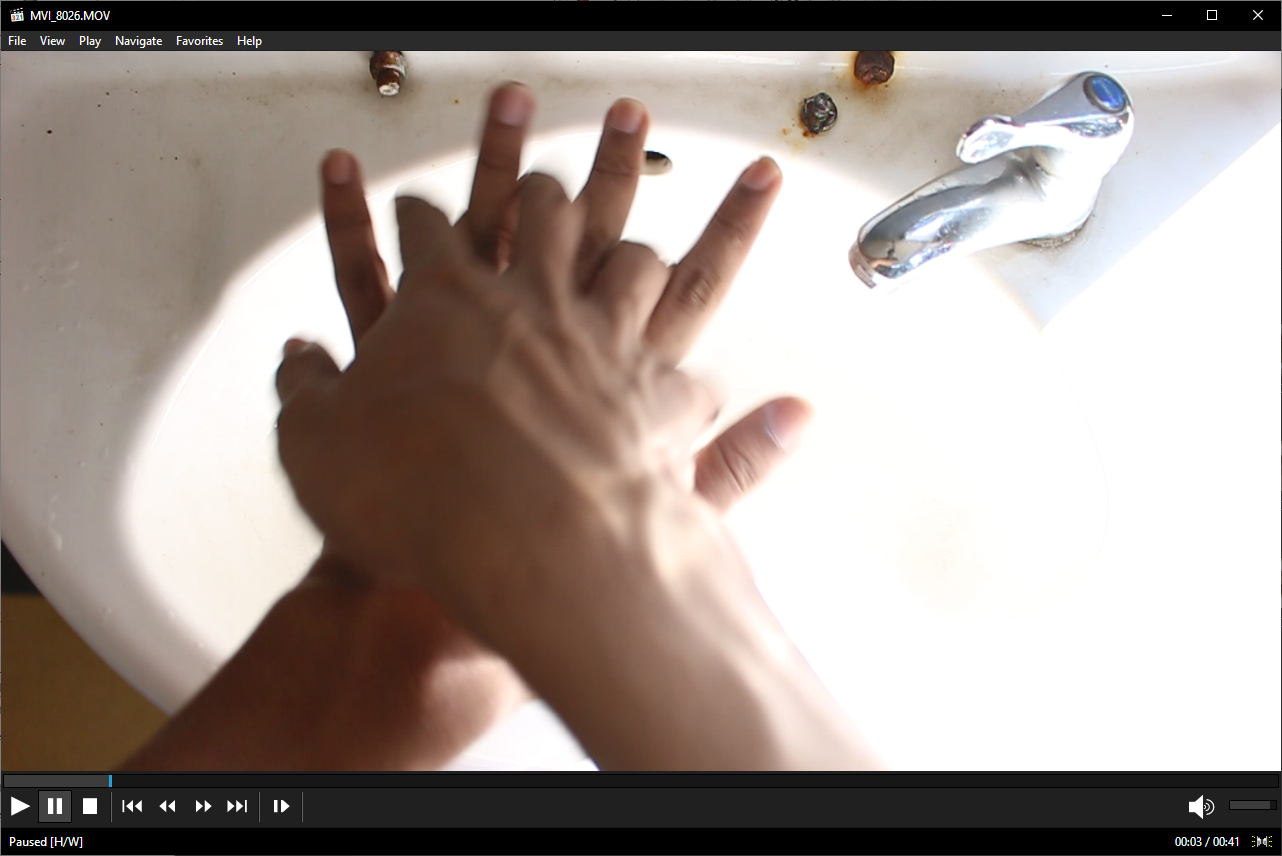
\includegraphics[width=0.8\columnwidth]{gambar/contohdslr2.png}
	\caption{Setup pengambilan dataset menggunakan DSLR}
	\label{fig:contohdslr}
\end{figure}

\section{Pengolahan Dataset}
\label{sec:pengolahandataset}

Pada pengolahan dataset, Dataset yang diambil dari kaggle diperiksa satu-persatu. Pada pemeriksaan ini, ditemukan kesalahan dalam struktural dataset tersebut. Struktur dataset kaggle diperbaiki agar sesuai dengan label nya. berberapa kesalahan pada struktur dataset kaggle ini antara lain gerakan tangan yang tertukar antara kanan dan kiri dan kesalahan peletakan dalam folder. Ditemukan pula kesalahan berupa "kontaminasi" gerakan yang berbeda pada satu video gerakan. Hal ini kemudian diperbaiki dengan membuang kontaminasi tersebut

Dataset yang diambil secara pribadi dari Webcam dan DSLR juga diperiksa. kontaminasi juga ditemukan akibat ketidaksengajaan pada proses perekaman dan turut dibersihkan. kemudian berberapa video dengan durasi yang terlalu lama di potong menjadi 2 video terpisah. Dataset ini kemudian di \textit{encoding} ulang untuk mempermudah proses training.

\section{Pengembangan Sistem}
\label{sec:pengembangansistem}

Pada tahap ini, sistem dikembangkan untuk dapat mengklasifikasikan gerakan cuci tangan. Sistem ini didasarkan oleh prinsip kerja \textit{Image Classification} berbasis CNN yang kemudian dilakukan movinf average dari outputnya agar dapat mengklasifikasikan sebuah gerakan dari hasil Image Classification tersebut.

Untuk membuat sistem klasifikasi yang dibutuhkan, digunakan Model EfficientNet sebagai \textit{base model}. Model ini digunakan karena kemampuannya melakukan Image Classification secara Effisien dimana hanya membutuhkan resource yang sedikit untuk mencapai Akurasi yang cukup tinggi dibandingkan model \textit{Transfer Learning} lainnya, seperti yang dijelaskan pada bagian \ref{sec:effnet}

Desain dari sistem klasifikasi pada penelitian ini terdiri dari berberapa tahapan yang harus dilalui. tahapan-tahapan tersebut adalah sebagai berikut:

\newpage
\begin{enumerate}[nolistsep]
	\item Frame Extraction
	\item Train \& Test Data Split
	\item Preprocessing
	\item Training
	\item Klasifikasi Frame
	\item Moving Average
\end{enumerate}

Tahapan-tahapan tersebut disusun bedarsarkan blok diagram yang dapat dilihat pada gambar \ref{fig:klasifikasi}

\begin{figure}[!ht]
	\centering
	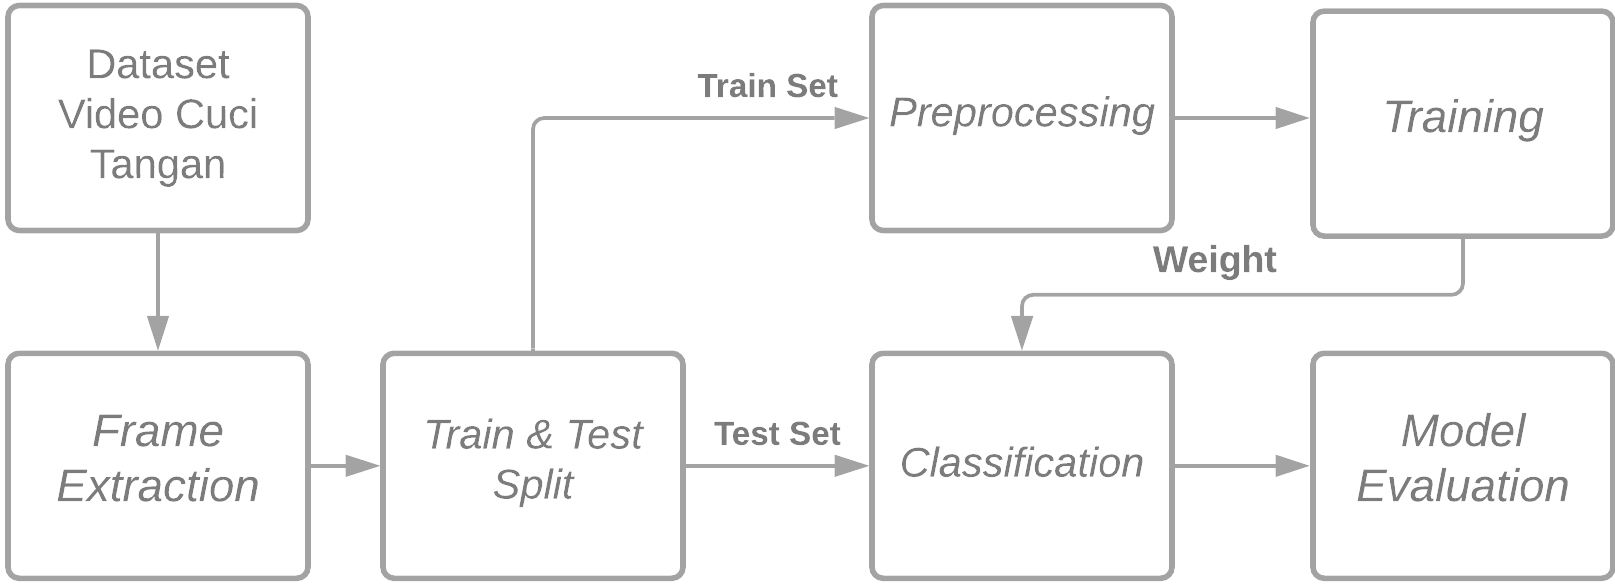
\includegraphics[width=1\columnwidth]{gambar/modelklasifikasi.png}
	\caption{Sistem Klasifikasi Gerakan Cuci Tangan}
	\label{fig:klasifikasi}
\end{figure}

\subsection{Frame Extraction}
\label{subsec:framextraction}

Pada tahap \textit{Frame Extraction}, Frame dari video di extract agar dapat diproses oleh model. Frame ini di extract secara random sebanyak 6000 frame untuk setiap class / label yang ada, hal ini dilakukan guna mendapatkan data yang beragam agar model yang sudah di training memiliki kemampun klasifikasi dengan akurasi yang cukup tinggi. Sampai disini, frame-frame tersebut masih terlalu besar untuk dapat di proses oleh EfficientNet-B0. EfficientNet-B0 hanya dapat memproses citra dalam resolusi 224 x 224 x 3, oleh karena itu frame-frame yang sudah di ekstraksi akan di \textit{resize} ke resolusi tersebut. Masing-masing frame yang sudah melalui tahap \textit{resize} kemudian akan dilabeli berdasarkan label pada video yang bersangkutan dan dimasukkan kedalam \textit{Numpy Array}.

\newpage
\subsection{Train \& Test Data Split}
\label{subsec:traintestsplit}

Pada tahap \textit{Train \& Test Data Split}, Array dari tahap \textit{Frame Extraction} kemudian akan dibagi kedalam \textit{Training Dataset} dan \textit{Test Dataset} dengan perbandingan 80 : 20. Training Dataset nantinya digunakan untuk melakukan training pada model sedangkan Test Dataset akan digunakan untuk mengevaluasi performa dari model yang sudah di training.

\subsection{Preprocessing}
\label{subsec:preprocessing}

Preprocessing ditempatkan sebagai bagian dari model. Citra pada Training Dataset akan di augmentasi agar memiliki bentuk yang lebih beragam. Augmentasi yang dilakukan diantaranya sebagai berikut:
\begin{itemize}
	\item \textit{\textbf{Random Rotation}}
	
	Random Rotation atau Rotasi Acak dilakukan guna mendapatkan hasil citra yang sudah di rotasi secara acak. Ini dilakukan agar model dapat mengklasifikasikan sebuah citra meski citra tersebut tidak tegak lurus.
	
	\item \textit{\textbf{Random Translation}}
	
	Random Translation atau Translasi Acak dilakukan guna mendapatkan citra yang posisinya sudah digeser secara acak. Ini dilakukan agar model dapat mengklasifikasikan citra walau citra tersebut sedikit bergeser dari posisi yang seharusnya
	
	\item \textit{\textbf{Random Flip}}
	
	Random Flip atau Pembalikan Acak dilakukan guna mendapatkan citra yang dimensinya sudah dibalik secara acak. Ini dilakukan agar model dapat mengklasifikasikan sebuah citra meskipun dimensinya sudah dibalik.
	
	\item \textit{\textbf{RandomContrast}}
	
	Random Contrast atau Pergeseran Kontras Acak dilakukan guna mendapat citra dengan kontras yang beragam. Ini dilakukan agar model dapat mengklasifikasikan citra dengan kontras yang beragam yang biasanya terjadi akibat efek pengambilan gambar pada situasi pencahayaan yang berbeda ataupun gambar yang berasal dari sensor kamera yang memiliki intensitas yang berbeda.
\end{itemize}

Tujuan utama dari preprocessing ini adalah supaya model yang sudah di training dapat mengenali fitur pada citra dengan lebih mudah dan memberikan hasil klasifikasi yang lebih akurat jika dibandingkan dengan model yang sama tanpa menggunakan preprocessing pada fase training nya.

Perlu diketahui pula, walaupun preprocessing ini ditempatkan sebagai bagian dari model, preprocessing ini hanya akan terjadi pada Training Dataset. Test Dataset maupun data lain yang sifatnya tidak mempengaruhi weight pada model tidak akan melalui tahap preprocessing ini.

\subsection{Training}
\label{subsec:training}

Model dasar yang digunakan pada sistem ini adalah EfficientNet-B0 \cite{cit:effnet} seperti yang dijelaskan pada bagian \ref{sec:effnet} dengan konfigurasi sebagai berikut:
\begin{lstlisting}[
language=Python,
caption={Konfigurasi EfficientNet},
label={lst:effnetconfig}
]
efnb = tf.keras.applications.EfficientNetB0(
	include_top=False,
	weights="efficientnetb0_notop.h5",
	input_shape=(224,224,3)
	)

for layer in efnb.layers[-20:]:
	if not isinstance(layer, layers.BatchNormalization):
		layer.trainable = True
\end{lstlisting} 

Karena gerakan mencuci tangan hanyalah sebagian kecil dari keseluruhan citra pada frame yang diklasifikasikan. Model ini dibantu dengan menggunakan weight checkpoint oleh NoisyStudent \cite{cit:noisy} guna mendapatkan akurasi yang cukup. Sebagian Layer dari Model \textit{Transfer Learning} EfficientNet ini juga diatur sebagai "trainable" agar model dapat mengenali gerakan tangan tersebut, yang bagi mesin/komputer, memiliki sedikit sekali perbedaan dengan frame lainnya pada satu video. Struktur Layer Pada Keseluruhan Model Klasifikasi ini dapat dilihat pada gambar \ref{fig:strukturmodel}

\begin{figure}[!ht]
	\centering
	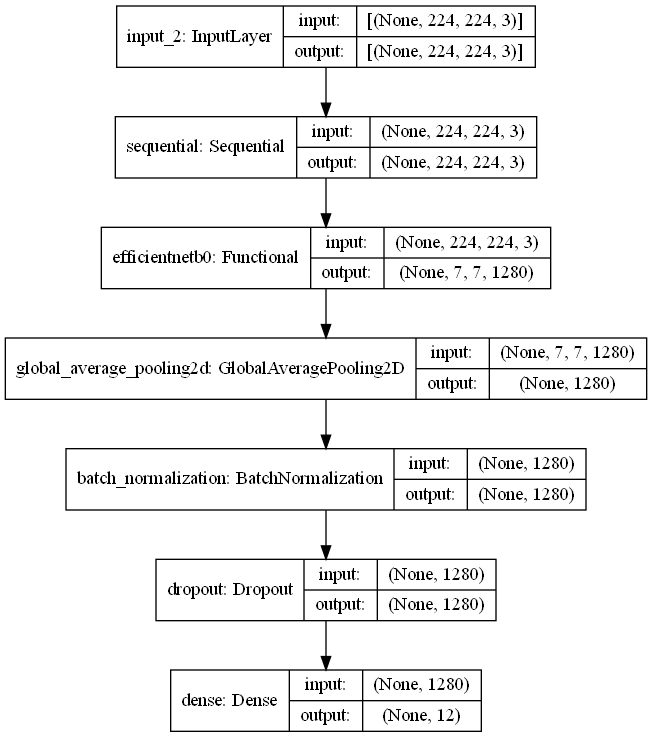
\includegraphics[width=1\columnwidth]{gambar/modelstructure.png}
	\caption{Struktur Model Klasifikasi Gerakan Cuci Tangan}
	\label{fig:strukturmodel}
\end{figure}

\newpage
Proses Training pada model ini dilakukan sebanyak 25 \textit{Epoch}. Pada tahap ini pula, 20\% dari dataset diambil untuk keperluan validasi. \textit{Optimizer Adam}, dengan \textit{Learning Rate} 0.001 digunakan untuk mengupdate bias pada Neural Network menggunakan hasil validasi pada setiap Epoch. Keseluruhan Konfigurasi Training dapat dilihat pada \textit{Code Listing} \ref{lst:callback}, \ref{lst:compile} dan \ref{lst:modelfit}

\newpage
\begin{lstlisting}[
	language=Python,
	caption={Training Callbacks},
	label={lst:callback}
	]
callbacks = [
	ReduceLROnPlateau(
	monitor='val_accuracy',
	mode='max',
	patience=7, 
	verbose=1,
	),
	
	EarlyStopping(
	monitor = 'val_loss', 
	mode='min',
	patience = 10, 
	restore_best_weights = True,
	verbose=1
	),
	
	ModelCheckpoint(
	'chkp/CHKP-{epoch:02d}-{val_accuracy:.2f}.h5',
	monitor='val_accuracy',
	mode='max',
	save_best_only = True,
	verbose=1
	)
	]
\end{lstlisting} 

\begin{lstlisting}[
	language=Python,
	caption={Konfigurasi pada model.compile},
	label={lst:compile}
	]
optimizers = tf.keras.optimizers.Adam(learning_rate=0.001)
model.compile(loss = 'categorical_crossentropy', optimizer = optimizers, metrics = ["accuracy"])
gc.collect()
\end{lstlisting} 

\begin{lstlisting}[
	language=Python,
	caption={Konfigurasi pada model.fit},
	label={lst:modelfit}
	]
model_training_history = model.fit(x = features_train, y = labels_train, epochs = 25, batch_size = 12 , shuffle = True, validation_split = 0.2, callbacks = callbacks)
gc.collect()
\end{lstlisting} 

\pagebreak
\subsection{Klasifikasi Frame}
\label{subsec:klasifikasiframe}

Setelah model berhasil di training maka akan didapatkan weight dari model tersebut, weight ini kemudian dapat digunakan pada tahap Klasifikasi Frame. Klasifikasi Frame dilakukan dengan menginput data berupa Video gerakan ke model yang sudah ditraining tanpa memberi pengaruh pada weight hasil training sebelumnya. Model kemudian akan memberikan output berupa prediksi dari setiap frame dan menyimpannya dalam bentuk array.

Pada tahap pengembangan sistem. data yang akan dimasukkan ke dalam \textit{pretrained} model tersebut adalah \textit{Test Dataset} yang didapat dari \textit{Train \& Test Data Split} pada bagian \ref{subsec:traintestsplit}. Model kemudian akan mengklasifikasikan dataset tersebut dan memberikan outputnya dalam bentuk array yang dapat digunakan pada tahap evaluasi model.

Untuk tahap testing, proses klasifikasi memiliki alur input data yang berbeda dimana data dalam bentuk sebuah video yang berisikan kombinasi urutan gerakan cuci tangan akan di ekstraksi ke dalam bentuk frame. Data ini tidak memiliki label seperti halnya dataset yang digunakan pada saat training kemudian akan dimasukkan ke dalam model. output dari klasifikasi ini akan nantinya digunakan pada tahap \textit{Moving Average}. Alur Klasifikasi pada tahap penggunaan ini dapat dilihat pada gambar \ref{fig:kerjasistem}

\begin{figure}[!ht]
	\centering
	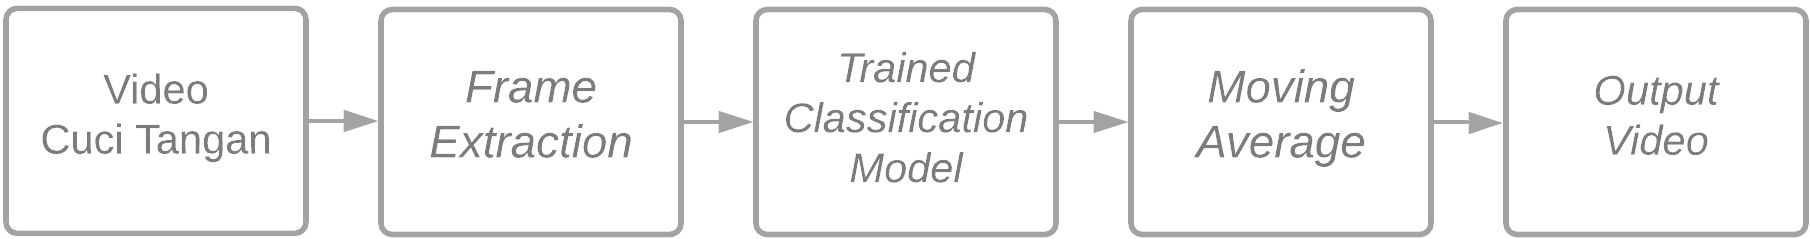
\includegraphics[width=0.9\columnwidth]{gambar/kerjasistem.png}
	\caption{Sistem Klasifikasi Gerakan Video Cuci Tangan}
	\label{fig:kerjasistem}
\end{figure}

\subsection{Moving Average}
\label{subsec:movingaverage}

Moving Average digunakan untuk menggambungkan dan "merata-ratakan" hasil klasifikasi gerakan dari output klasifikasi frame. Ini digunakan agar output dari sistem ini adalah berupa hasil klasifikasi gerakan per satuan waktu. Pada tahap ini, ditentukan \textit{Window Size} yang didefinisikan dengan \textit{Deque (Double-ended Queue)}. Window Size dapat diatur sesuai kebutuhan dengan minimal 24 frame atau sesuai dengan \textit{FPS} dari Video Input. Semakin panjang Deque yang digunakan, maka akan semakin lama proses Moving Average pada setiap gerakan. 

Hasil dari Moving Average dituliskan pada frame-frame yang diklasifikasikan. Pada bagian outputnya, frame-frame tersebut akan disatukan kembali dan di tampilkan dalam wujud video hasil klasifikasi. Contoh Hasil klasifikasi beserta teks keterangannya dapat dilihat pada gambar \ref{fig:contohhasil}
\begin{figure}[!ht]
	\centering
	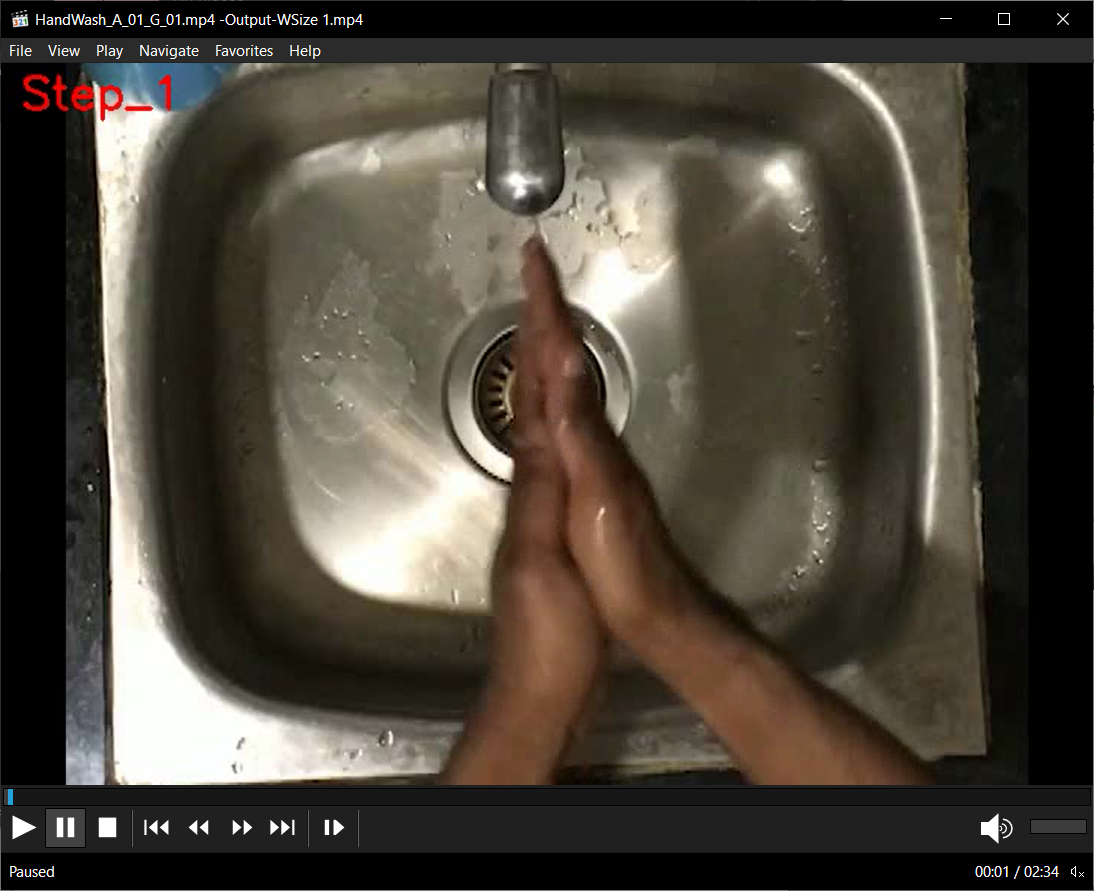
\includegraphics[width=0.9\columnwidth]{gambar/contohhasilklasifikasi.png}
	\caption{Contoh Hasil Klasifikasi}
	\label{fig:contohhasil}
\end{figure}
